

% Pattern Info
 
\tikzset{
pattern size/.store in=\mcSize, 
pattern size = 5pt,
pattern thickness/.store in=\mcThickness, 
pattern thickness = 0.3pt,
pattern radius/.store in=\mcRadius, 
pattern radius = 1pt}
\makeatletter
\pgfutil@ifundefined{pgf@pattern@name@_hy82zy3w3}{
\pgfdeclarepatternformonly[\mcThickness,\mcSize]{_hy82zy3w3}
{\pgfqpoint{-\mcThickness}{-\mcThickness}}
{\pgfpoint{\mcSize}{\mcSize}}
{\pgfpoint{\mcSize}{\mcSize}}
{
\pgfsetcolor{\tikz@pattern@color}
\pgfsetlinewidth{\mcThickness}
\pgfpathmoveto{\pgfpointorigin}
\pgfpathlineto{\pgfpoint{0}{\mcSize}}
\pgfusepath{stroke}
}}
\makeatother
\tikzset{every picture/.style={line width=0.75pt}} %set default line width to 0.75pt        

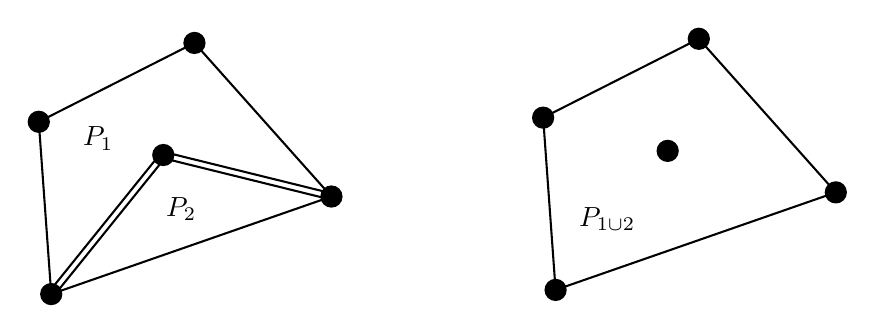
\begin{tikzpicture}[x=0.75pt,y=0.75pt,yscale=-1,xscale=1]
%uncomment if require: \path (0,300); %set diagram left start at 0, and has height of 300

%Shape: Circle [id:dp0903854075610232] 
\draw  [fill={rgb, 255:red, 0; green, 0; blue, 0 }  ,fill opacity=1 ] (106.3,114.85) .. controls (106.3,112.17) and (108.47,110) .. (111.15,110) .. controls (113.83,110) and (116,112.17) .. (116,114.85) .. controls (116,117.53) and (113.83,119.7) .. (111.15,119.7) .. controls (108.47,119.7) and (106.3,117.53) .. (106.3,114.85) -- cycle ;
%Shape: Circle [id:dp3184910134932345] 
\draw  [fill={rgb, 255:red, 0; green, 0; blue, 0 }  ,fill opacity=1 ] (112.3,197.85) .. controls (112.3,195.17) and (114.47,193) .. (117.15,193) .. controls (119.83,193) and (122,195.17) .. (122,197.85) .. controls (122,200.53) and (119.83,202.7) .. (117.15,202.7) .. controls (114.47,202.7) and (112.3,200.53) .. (112.3,197.85) -- cycle ;
%Shape: Circle [id:dp5872048719836919] 
\draw  [fill={rgb, 255:red, 0; green, 0; blue, 0 }  ,fill opacity=1 ] (247.3,150.85) .. controls (247.3,148.17) and (249.47,146) .. (252.15,146) .. controls (254.83,146) and (257,148.17) .. (257,150.85) .. controls (257,153.53) and (254.83,155.7) .. (252.15,155.7) .. controls (249.47,155.7) and (247.3,153.53) .. (247.3,150.85) -- cycle ;
%Shape: Circle [id:dp7591641248768922] 
\draw  [fill={rgb, 255:red, 0; green, 0; blue, 0 }  ,fill opacity=1 ] (181.3,76.85) .. controls (181.3,74.17) and (183.47,72) .. (186.15,72) .. controls (188.83,72) and (191,74.17) .. (191,76.85) .. controls (191,79.53) and (188.83,81.7) .. (186.15,81.7) .. controls (183.47,81.7) and (181.3,79.53) .. (181.3,76.85) -- cycle ;
%Shape: Circle [id:dp7762987079639629] 
\draw  [fill={rgb, 255:red, 0; green, 0; blue, 0 }  ,fill opacity=1 ] (166.3,130.85) .. controls (166.3,128.17) and (168.47,126) .. (171.15,126) .. controls (173.83,126) and (176,128.17) .. (176,130.85) .. controls (176,133.53) and (173.83,135.7) .. (171.15,135.7) .. controls (168.47,135.7) and (166.3,133.53) .. (166.3,130.85) -- cycle ;
%Shape: Circle [id:dp7626801331888498] 
\draw  [fill={rgb, 255:red, 0; green, 0; blue, 0 }  ,fill opacity=1 ] (349.3,112.85) .. controls (349.3,110.17) and (351.47,108) .. (354.15,108) .. controls (356.83,108) and (359,110.17) .. (359,112.85) .. controls (359,115.53) and (356.83,117.7) .. (354.15,117.7) .. controls (351.47,117.7) and (349.3,115.53) .. (349.3,112.85) -- cycle ;
%Shape: Circle [id:dp6435093773617909] 
\draw  [fill={rgb, 255:red, 0; green, 0; blue, 0 }  ,fill opacity=1 ] (355.3,195.85) .. controls (355.3,193.17) and (357.47,191) .. (360.15,191) .. controls (362.83,191) and (365,193.17) .. (365,195.85) .. controls (365,198.53) and (362.83,200.7) .. (360.15,200.7) .. controls (357.47,200.7) and (355.3,198.53) .. (355.3,195.85) -- cycle ;
%Shape: Circle [id:dp23520259436348545] 
\draw  [fill={rgb, 255:red, 0; green, 0; blue, 0 }  ,fill opacity=1 ] (490.3,148.85) .. controls (490.3,146.17) and (492.47,144) .. (495.15,144) .. controls (497.83,144) and (500,146.17) .. (500,148.85) .. controls (500,151.53) and (497.83,153.7) .. (495.15,153.7) .. controls (492.47,153.7) and (490.3,151.53) .. (490.3,148.85) -- cycle ;
%Shape: Circle [id:dp5139999912619062] 
\draw  [fill={rgb, 255:red, 0; green, 0; blue, 0 }  ,fill opacity=1 ] (424.3,74.85) .. controls (424.3,72.17) and (426.47,70) .. (429.15,70) .. controls (431.83,70) and (434,72.17) .. (434,74.85) .. controls (434,77.53) and (431.83,79.7) .. (429.15,79.7) .. controls (426.47,79.7) and (424.3,77.53) .. (424.3,74.85) -- cycle ;
%Shape: Circle [id:dp9128853181814609] 
\draw  [fill={rgb, 255:red, 0; green, 0; blue, 0 }  ,fill opacity=1 ] (409.3,128.85) .. controls (409.3,126.17) and (411.47,124) .. (414.15,124) .. controls (416.83,124) and (419,126.17) .. (419,128.85) .. controls (419,131.53) and (416.83,133.7) .. (414.15,133.7) .. controls (411.47,133.7) and (409.3,131.53) .. (409.3,128.85) -- cycle ;
%Straight Lines [id:da9543502559927777] 
\draw    (111.15,114.85) -- (117.15,197.85) ;
%Straight Lines [id:da6236204803411575] 
\draw    (111.15,114.85) -- (186.15,76.85) ;
%Straight Lines [id:da36073679376855783] 
\draw    (186.15,76.85) -- (252.15,150.85) ;
%Straight Lines [id:da5089280650914181] 
\draw    (171.51,129.39) -- (252.51,149.39)(170.79,132.31) -- (251.79,152.31) ;
%Straight Lines [id:da9757972098601457] 
\draw (172.32,131.79) -- (118.32,198.79)(169.98,129.91) -- (115.98,196.91) ;
%Straight Lines [id:da2697882015737454] 
\draw    (252.15,150.85) -- (117.15,197.85) ;
%Straight Lines [id:da45150527483296576] 
\draw    (354.15,112.85) -- (360.15,195.85) ;
%Straight Lines [id:da030554361443556277] 
\draw    (354.15,112.85) -- (429.15,74.85) ;
%Straight Lines [id:da1930137132355716] 
\draw    (429.15,74.85) -- (495.15,148.85) ;
%Straight Lines [id:da9231067498266883] 
\draw    (360.15,195.85) -- (495.15,148.85) ;

% Text Node
\draw (131,115.85) node [anchor=north west][inner sep=0.75pt]   [align=left] {$\displaystyle P_{1}$};
% Text Node
\draw (171,149.85) node [anchor=north west][inner sep=0.75pt]   [align=left] {$\displaystyle P_{2}$};
% Text Node
\draw (370,154.85) node [anchor=north west][inner sep=0.75pt]   [align=left] {$\displaystyle P_{1\cup 2}$};


\end{tikzpicture}
